\section{WSNet}

The following section describes the assessment and evaluation of WSNet. This starts with an implementation of the tested models and with checking for deviations between described methods and available code. Following that, several experiments are performed to assess the algorithm in more detail and to check its robustness.

\subsection{Code availability and reproduction of the results}

Although the code for WSNet \cite{Oota_2023_WACV} is stated to be publicly available, a closer inspection of the linked GitHub repository shows that this is only partially the case. A lack of documentation makes using the code hard, especially since it seems to contain multiple errors, making it only suitable as a base for new code.

In this project's scope, the code was used to create runnable models again. Unfortunately, the classes of the wounds are not available, making it impossible to perform pre-training as described in the original paper \cite{Oota_2023_WACV}. In total, there are eight models available: A local model and a combined global-local model for each of the segmentation models: Unet, PSPNet, FPN, and LinkNet. The Python library used for the segmentation models is \texttt{segmentation\_models} \cite{SegmentationModels}. The implementation process showed some differences from the described model architecture. In particular, it was claimed that the wound images were split up in parts of 48\,px times 48\,px. However, three of the four models, all besides PSPNet, only allow input sizes divisible by 32, and the code in GitHub showed a size of 64\,px was used. Another difference between the available code and the paper is that it is claimed that augmentation is not performed on the test images, which is not the case.

Information about the training, validation and test set size is not given in the paper or code. However, the code reveals that the train and validation sets were just the first x\,\% of the dataset, and no randomisation was used to separate the test set as it is usually done. In this project's scope, a split of 70\,\% training, 15\,\% validation and 15\,\% test data is used.

Because the data training for the wound-specific pre-training is not available, the results can only be compared for imagenet pre-training. An important aspect is, that mobilenet has no pretrained weights for images with the size of the patches and the default size of 224x224\,px is used instead, which might impact results negatively.

\subsection{Comparison of the achieved performance}

\begin{table}[htb!]
	\centering
	\begin{tabular}{l||c | c | c | c | c | c | c | c|}
	& \multicolumn{2}{|c|}{Unet} & \multicolumn{2}{|c|}{LinkNet} & \multicolumn{2}{|c|}{PSPNet} & \multicolumn{2}{|c|}{FPN} \\
	\hline
	& IoU & Dice & IoU & Dice & IoU & Dice & IoU & Dice \\
	\hline\hline
	\textbf{Local model} & 0.359 & 0.523 & 0.398 & 0.564 & 0.373 & 0.538 & 0.408 & 0.574 \\	
	\textbf{Global model} & 0.504 & 0.668 & 0.631 & 0.772 & 0.458 & 0.627 & 0.632 & 0.772 \\
	\textbf{Global-Local model} & 0.495 & 0.658 & 0.618 & 0.763 & 0.476 & 0.642 & 0.612 & 0.758\\
	\end{tabular}
	\caption{IoU-Scores and Dice Coefficients for the four different models with each Global-Local, Global and Local architecture. The backbone used is mobilenet.}
\end{table}

\begin{table}[htb!]
	\centering
	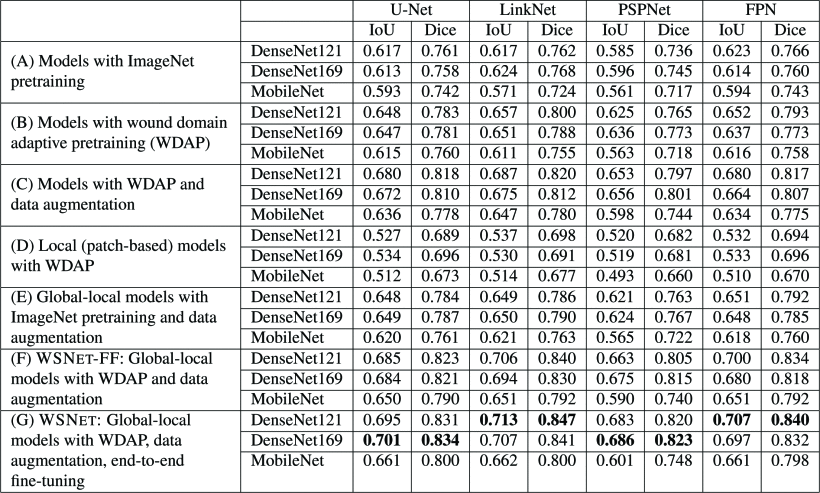
\includegraphics[width=\textwidth]{fig/wsnet-results.png}
	\caption{Results reported by \citeauthor{Oota_2023_WACV} \cite{Oota_2023_WACV}.}
\end{table}

\begin{itemize}
	\item results are comparable with results reported in paper, slightly lower scores
	\item e.g. Unet IoU score 0.495 with my code, 0.620 in paper (dice score 0.761 vs 0.658)
	\item others are closer (LinkNet 0.618 from me vs 0.621 in paper, dice 0.763 in paper and for me)
	\item maybe differences in training size
	\item most important thing: the global-local model does not improve about global model (or at least less than reported in paper)
	\item but they are still way more computationally expensive because you need to train two models instead of one
	\item as discussed before, an improvement indicates that something is going on with 48\,px context size
	\item the results reported by \citeauthor{Oota_2023_WACV} are shown in figure
\end{itemize}

\subsection{Experiments with the activation function}

\begin{itemize}
	\item code shows use of sigmoid as activation function
	\item literature of the model reports ReLU more frequently, thus it was tested as alternative to sigmoid
	\item no clear trend of one being clearly better for all models and architectures
\end{itemize}

\begin{table}[htb!]
	\centering
	\begin{tabular}{l | c ||c | c || c | c || c | c || c | c||}
	& & \multicolumn{2}{|c||}{Unet} & \multicolumn{2}{|c||}{LinkNet} & \multicolumn{2}{|c||}{PSPNet} & \multicolumn{2}{|c||}{FPN} \\
	\hline
	& Activation & IoU & Dice & IoU & Dice & IoU & Dice & IoU & Dice \\
	\hline\hline
	\multirow{2}{*}{\textbf{Local model}} & Sigmoid & 0.359 & 0.523 & 0.398 & 0.564 & 0.373 & 0.538 & 0.408 & 0.574 \\
	& ReLU & 0.398 & 0.565 & 0.396 & 0.561 & 0.372 & 0.536 & 0.380 & 0.546 \\
	\hline
	\multirow{2}{*}{\textbf{Global model}} & Sigmoid & 0.504 & 0.668 & 0.631 & 0.772 & 0.458 & 0.627 & 0.632 & 0.772 \\
	& ReLU & 0.513 & 0.676 & 0.509 & 0.672 & 0.463 & 0.631 & 0.505 & 0.669 \\
	\hline
	\multirow{2}{*}{\textbf{Global-Local model}} & Sigmoid & 0.495 & 0.658 & 0.618 & 0.763 & 0.476 & 0.642 & 0.612 & 0.758\\
	& ReLU & 0.498 & 0.662 & 0.588 & 0.738 & 0.569 & 0.724 & 0.610 & 0.756 \\
	\end{tabular}
	\caption{IoU-Scores and Dice Coefficients for the four different models with each Global-Local, Global and Local architecture compared for the Sigmoid and ReLU activation function.}
	\label{table:sigmoid-relu-comparison}
\end{table}


\subsection{Combination of different architectures}

\begin{itemize}
	\item used model architectures localize signals differently by design
	\item if the patch size really does play a significant role, maybe it makes sense to combine different architecture sizes?
\end{itemize}

\begin{table}[htb!]
	\centering
	\begin{tabular}{c|c| c| c}
		Global Model & Local Model & IoU & Dice \\ \hline\hline
		\multirow{4}{*}{U-Net} & U-Net & 0.495 & 0.658\\
		 & LinkNet  & 0.602 & 0.749 \\
		 & PSPNet & 0.607 & 0.753 \\
		 & FPN & 0.613 & 0.757 \\\hline
		 \multirow{4}{*}{LinkNet} & LinkNet & 0.618 & 0.763 \\
		 & U-Net  & 0.633 & 0.774 \\
		 & PSPNet & 0.612 & 0.757 \\
		 & FPN & 0.613 & 0.758 \\\hline
		 \multirow{4}{*}{PSPNet} & PSPNet & 0.476 &  0.642\\
		 & U-Net  & 0.554 & 0.711 \\
		 & LinkNet & 0.576 & 0.729 \\
		 & FPN & 0.580 & 0.732 \\\hline
		 \multirow{4}{*}{FPN} & FPN & 0.612 & 0.758 \\
		 & U-Net  & 0.605 & 0.752 \\
		 & LinkNet & 0.585 & 0.735 \\
		 & PSPNet & 0.627 & 0.769 \\\hline
	\end{tabular}	
\end{table}


\subsection{Assessing the Robustness}

As already discussed, one problem of wound segmentation is the diversity of available wound images. A segmentation should therefore be robust and work for a variety of image types. To asses the robustness of the models, two experiments were performed: Testing the performance on augmented images and testing the performances on another data set without re-training the models.

\subsubsection{Robustness against image augmentations}

\begin{itemize}
	\item augmentations commonly performed to improve robustness of models
	\item can also be used to access robustness of the resulting model
	\item for clinical application, lightning and size might vary between images
	\item batch normalization might further increase this problem (TODO: search references)
	\item what have I done: a trained model should ideally be able to deal with other kinds of data it is not trained on
	\item for this purpose different type of augmentations performed on test set
	\item tensorflow image functions were used for this purpose
	\item implemented augemtations and why
	\item embed in black box: test against changes in size, most likely the case in real scenarios. Also, the model needs a square input and images might not always be square and rescaling and padding in black background is likely solution for images in other formats
	\item change brightness, saturation, contrast: lightning conditions might change, different camera, etc. all of those things can influence colour and lightning
\end{itemize}

\begin{table}[htb!]
	\centering
	\begin{tabular}{l | c ||c | c || c | c || c | c || c | c||}
	& & \multicolumn{2}{|c||}{Unet} & \multicolumn{2}{|c||}{LinkNet} & \multicolumn{2}{|c||}{PSPNet} & \multicolumn{2}{|c||}{FPN} \\
	\hline
	& Augmentation & IoU & Dice & IoU & Dice & IoU & Dice & IoU & Dice \\
	\hline\hline
	\multirow{5}{*}{\textbf{Local model}} & - & 0.359 & 0.523 & 0.398 & 0.564 & 0.373 & 0.538 & 0.408 & 0.574 \\
	& Embed & 0.365 & 0.528 & 0.378 & 0.545 & 0.373 & 0.534 & 0.383 & 0.550\\
	& Brightness & 0.341 & 0.503 & 0.391 & 0.557 & 0.348 & 0.510 & 0.417 & 0.583\\
	& Contrast & 0.297 & 0.454 & 0.286 & 0.442 & 0.270 & 0.422 & 0.206 & 0.338\\
	& Saturation & 0.310 & 0.470 & 0.284 & 0.396 & 0.245 & 0.390 & 0.211 & 0.346\\
	\hline
	\multirow{5}{*}{\textbf{Global model}} & - & 0.504 & 0.668 & 0.631 & 0.772 & 0.458 & 0.627 & 0.632 & 0.772 \\
	& Embed & 0.400 & 0.566 & 0.438 & 0.607 & 0.333 & 0.497 & 0.454 & 0.622\\
	& Brightness & 0.500 & 0.663 & 0.629 & 0.770 & 0.452 & 0.620 & 0.625 & 0.767\\
	& Contrast & 0.404 & 0.573 & 0.539 & 0.699 & 0.334 & 0.499 & 0.562 & 0.718\\
	& Saturation & 0.420 & 0.586 & 0.475 & 0.641 & 0.346 & 0.511 & 0.441 & 0.609\\
	\hline
	\multirow{5}{*}{\textbf{Global-Local model}} & - & 0.495 & 0.658 & 0.618 & 0.763 & 0.476 & 0.642 & 0.612 & 0.758\\
	& Embed & 0.372 & 0.541 & 0.451 & 0.619 & 0.393 & 0.559 & 0.375 & 0.542\\
	& Brightness & 0.495 & 0.659 & 0.613 & 0.759 & 0.465 & 0.632 & 0.604 & 0.751\\
	& Contrast & 0.408 & 0.577& 0.545 & 0.704 & 0.414 & 0.583 & 0.503 & 0.666\\
	& Saturation & 0.402 & 0.570 & 0.491 & 0.657 & 0.387 & 0.555 & 0.490 & 0.654\\
	\end{tabular}
	\caption{IoU-Scores and Dice Coefficients for the four different models with each Global-Local, Global and Local architecture compared for different augmentations on the test images.}
	\label{table:dataset-comparison}
\end{table}

\begin{itemize}
	\item brightness change influences performance the least
	\item local models generally worst
	\item embed did not generally impacts global-local model the most, but for fpn, it is significantly worse than when just using a global model
\end{itemize}

\subsubsection{Performance on an unseen data set}

\begin{itemize}
	\item data set of Foot Ulcer Segmentation Challenge 2021 \cite{Wang2020} used that was mentioned in section \ref{sec:data-sets}
	\item data is loaded, resized to 192x192\,px and then tested with the already trained models
	\item results are displayed together with the original data set from WSNet in table \ref{table:dataset-comparison}.
\end{itemize}


\begin{table}[htb!]
	\centering
	\begin{tabular}{l | c ||c | c || c | c || c | c || c | c||}
	& & \multicolumn{2}{|c||}{Unet} & \multicolumn{2}{|c||}{LinkNet} & \multicolumn{2}{|c||}{PSPNet} & \multicolumn{2}{|c||}{FPN} \\
	\hline
	& Data set & IoU & Dice & IoU & Dice & IoU & Dice & IoU & Dice \\
	\hline\hline
	\multirow{2}{*}{\textbf{Local model}} & WSNet & 0.359 & 0.523 & 0.398 & 0.564 & 0.373 & 0.538 & 0.408 & 0.574 \\
	& DFUC & 0.262 & 0.411 & 0.203 & 0.335 & 0.231 & 0.372 & 0.231 & 0.372\\
	\hline
	\multirow{2}{*}{\textbf{Global model}} & WSNet & 0.504 & 0.668 & 0.631 & 0.772 & 0.458 & 0.627 & 0.632 & 0.772 \\
	& DFUC & 0.214 & 0.350 & 0.276 & 0.428 & 0.155 & 0.265 & 0.238 & 0.380\\
	\hline
	\multirow{2}{*}{\textbf{Global-Local model}} & WSNet & 0.495 & 0.658 & 0.618 & 0.763 & 0.476 & 0.642 & 0.612 & 0.758\\
	& DFUC & 0.201 & 0.330 & 0.181 & 0.304 & 0.181 & 0.304 & 0.215 & 0.349\\
	\end{tabular}
	\caption{IoU-Scores and Dice Coefficients for the four different models with each Global-Local, Global and Local architecture compared for the WSNet and the Diabetes Foot Ulcer Challenge (DFUC) 2021 data.}
	\label{table:dataset-comparison}
\end{table}

\begin{itemize}
	\item worsens performance by huge amount for every model
	\item probably training on mix needed but no time in the scope of the project
	\item means results are not directly transferable to new models
\end{itemize}
